% Kozierok, ch. 20
\chapter[IP classless addressing -- CIDR or supernetting]{IP classless addressing -- classless inter-domain routing (CIDR) or supernetting}
\label{chap:kozierok-ch20}

As the Internet began to grow dramatically, three main problems arose
with the original classful addressing scheme described in the previous
chapters. These difficulties were addressed partially through subnet
addressing, which provides more flexibility for the administrators of
individual networks on an Internet. Subnetting, however, doesn't really
tackle the problems in general terms. Some of these issues remain due to
the use of classes even with subnets.

While development began on version 6 of the Internet Protocol
(IPv6; see \vref{chap:ipv6}) and its roomy 128-bit
addressing system in the mid-1990s, developers recognized that it would take many years before widespread deployment of IPv6 would be possible.
In order to extend the life of IPv4 until the newer version could be completed, it was necessary to take a new approach to addressing IPv4 devices.
This new system calls for eliminating the notion of address classes entirely, creating a new {\emph{classless addressing}} scheme sometimes called \emph{classless inter-domain routing} (CIDR).

In this chapter, I describe modern classless IP addressing. I begin with
an overview of the concepts behind classless addressing and the idea
behind {\emph{supernetting}}, including why it was created and what its
advantages and disadvantages are. I then define
CIDR and
describe how the system works in more detail, including the notation
used for address blocks. I list each of the CIDR address block sizes and
show how they relate to the older class A, B, and C networks. I conclude
with a CIDR addressing example that's similar to the examples in
\cref{chap:kozierok-ch19}, but this one focuses on CIDR
and is a bit more condensed.

Subnet addressing was an important development in the evolution of IP
addressing, because it solved some important issues with the
conventional, two-level class-based addressing scheme. Subnetting's
contribution to flexibility in IP addressing was to allow each network
to have its own two-level hierarchy, thereby giving the administrator of
each network the equivalent of an Internet within the Internet.

When you looked at the advantages of subnetting in
\cref{chap:kozierok-ch18}, you saw that subnetting was
local within each organization and invisible to other organizations.
This is an advantage in that it lets each organization tailor its
network without other groups having to worry about the details of how
this is done. Unfortunately, this invisibility also represents a key
{\emph{disadvantage}} of subnetted classful addressing: It cannot
correct the fundamental inefficiencies associated with that type of
addressing, because organizations are still assigned address blocks
based on classes.



\section{The main problem with classful addressing}

A key weakness of the subnetting system is its low
granularity. A
class B address block contains a very large number of addresses
(65,534), but a class C block has only a relatively small number (254).
There are many thousands of medium-sized organizations that need more
than 254 IP addresses, but a small percentage of these needs 65,534 or
anything even close to it. (The lack of a good match to a medium-sized
organization with 5,000 hosts is illustrated in \vref{fig:problem-with-classful}.)
When setting up their networks, these companies and groups would tend to request class B
address blocks and not class C blocks, because they needed more than 254
hosts, without considering how many of the 65,000-odd addresses they
really would use.

Due to how the classes of the older system were designed, there are over
two million class C address blocks, but only 16,384 class B networks.
While 16,384 seems like a lot at first glance, there are millions of
organizations and corporations around the world.
Class B allocations were being consumed at a rapid pace, while the smaller class C networks were relatively unused.

The folks handing out Internet addresses needed a way to better utilize
the address space so that it would not run out before the transition to
IPv6. Subnetting didn't help a great deal with this problem. Why?
Because it only works {\emph{within}} the classful address blocks. If an
organization needing 2,000 IP addresses requested a class B block, they
could use subnetting to more efficiently manage their block. However,
subnetting could do nothing about the fact that this organization would
never use over 62,000 of the addresses in its block -- about 97 percent
of their allocated address space.

The only solution to this would be to convince -- or at worst case,
force -- companies to use many smaller class C blocks instead of wasting
the bulk of a class B assignment. Many organizations resisted this due
to the complexity involved, and this caused the other main problem that
subnetting didn't correct: the growth of Internet routing tables.
Replacing one class B network with 10 class C networks means ten times
as many entries for routers to maintain.

\section{The solution: eliminate address classes}

It was clear that as long as there were only three sizes of networks,
the allocation efficiency problem could never be properly rectified. The
solution was to get rid of the classes completely, in favor of a
{\emph{classless}}
allocation scheme. This system would solve both of the main problems
with classful addressing: inefficient address space use and the
exponential growth of routing tables.

This system was developed in the early 1990s and formalized in 1993 in
RFCs 1517, 1518, 1519, and 1520.
The technology was called \emph{classless inter-domain routing} (CIDR).
Despite this name, the scheme deals with both addressing and routing matters, since they are inextricably linked.

The idea behind CIDR is to adapt the concept of subnetting a single
network to the entire Internet. In essence, classless addressing means
that instead of breaking a particular network into subnets, you can
aggregate networks into larger ``supernets.''
CIDR is sometimes called {\emph{supernetting}} for this reason: It applies the principles of
subnetting to larger networks. It is this aggregation of networks into
supernets that allowed CIDR to resolve the problem of growing Internet
routing tables.

Of course, if you are going to apply subnetting concepts to the entire
Internet, you need to be able to have subnets of different sizes. After
all, that's one of the primary goals in eliminating the classes. So,
more accurately, CIDR is an Internet-wide application of not just
regular one-level subnetting, but of variable-length subnet masking (VLSM), introduced in \cref{chap:kozierok-ch18}.
Just as VLSM allows you split a network as many times as you want to create subnets, sub-subnets, and sub-sub-subnets,
CIDR lets you do this with the entire Internet, as many times as needed.


\begin{keyconcept}
\emph{Classless inter-domain routing} (CIDR) is a system of IP addressing and routing that solves the many problems of
classful addressing by eliminating fixed address classes in favor of a flexible, multiple-level, hierarchical structure of networks of varying sizes.
\end{keyconcept}

\section{The many benefits of classless addressing and routing}

CIDR provides numerous advantages over the classful addressing scheme, whether or not subnetting is used:

\begin{description}
   \item[Efficient address space allocation]
      Instead of allocating addresses in fixed-size blocks of low granularity, under CIDR, addresses are allocated in sizes of any binary multiple.
      So a company that needs 5,000 addresses can be assigned a block of 8,190 instead of 65,534, as shown in \protect\hyperlink{ch20.htmlux5cux23classless_addressing_cidr_solves_the_gra}{Figure~20-1}.
      Or to think of it another way, the equivalent of a single class B network can be shared among eight companies that each need 8,190 or fewer IP addresses.

   \item[Elimination of class imbalances]
      There are no more class A, B, and C networks, so there is no problem with some portions of the address space being widely used while others are neglected.

   \item[Efficient routing entries]
      CIDR's multiple-level hierarchical structure allows a small number of routing entries to represent a large number of networks.
      Network descriptions can be aggregated and represented by a single entry.
      Since CIDR is hierarchical, the detail of lower-level, smaller networks can be hidden from routers that move traffic between large groups of networks.
      %This is discussed more completely in \protect\hyperlink{ch23.html}{Chapter~23}, which covers IP routing issues.

   \item[No separate subnetting method]
      CIDR implements the concepts of subnetting within the Internet itself.
      An organization can use the same method used on the Internet to subdivide its internal network into subnets of arbitrary complexity,
      without needing a separate subnetting mechanism.
\end{description}


\begin{figure}
   \centering
   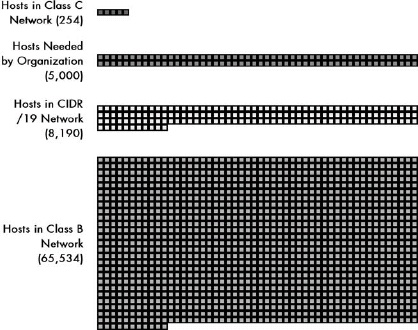
\includegraphics[width=.9\textwidth]{images/cidr-solves-granularity.jpg}
   \caption
      [Classless addressing (CIDR) solves the granularity problem]
      {Classless addressing (CIDR) solves the granularity problem --
      \vref{fig:problem-with-classful} illustrates the primary problem with classful addressing:
      the great distance between the size of class B and class C networks.
      CIDR solves this issue by allowing any number of bits to be used for the network ID.
      In the case of an organization with 5,000 hosts, a /19 network with 8,190 hosts can be assigned.
      This reduces the address space waste for such an organization by about 95 percent.}
   \label{fig:cidr-solves-granularity}
\end{figure}

Since the main benefit of classful addressing was its simplicity, it's
no surprise that the main drawback of CIDR is its greater complexity.
One issue is that it is no longer possible to determine, by looking at
the first octet, how many bits of an IP address represent the network ID
and how many represent the host ID. A bit more care needs to be used in
setting up routers as well, to make sure that routing is accomplished
correctly.

When you first looked at IP addressing in \cref{chap:kozierok-ch17},
you saw that IP addresses were designed to be divided into a network identifier (network ID) and host identifier (host ID).
Then, when subnets were introduced, you ``stole'' bits from the host ID to create a subnet ID, giving the IP address a total of three hierarchical levels.
With VLSM, you further subnetted the subnets, taking more bits from the host ID to give you a multiple-level hierarchy with sub-subnets,
sub-sub-subnets, and so forth.

In a classless environment, you completely change how you look at IP
addresses by applying VLSM concepts not just to one network, but to the
entire Internet. In essence, the Internet becomes just one giant network
that is subnetted into a number of large blocks. Some of these large
blocks are then broken down into smaller blocks, which can in turn be
broken down further. This breaking down can occur multiple times,
allowing you to split the ``pie'' of Internet addresses into slices of
many different sizes to suit the needs of the organization.

As the name implies, classless addressing completely eliminates the
prior notions of classes. There are no more class A, B, and C blocks
that are divided by the first few bits of the address.
Instead, under CIDR, all Internet blocks can be of arbitrary size. Instead of having all networks use 8 (class A), 16 (class B),
or 24 (class C) bits for the network ID, you can have large networks with, say, 13 bits for the network ID
(leaving 19 bits for the host ID), or very small ones that use 28 bits
for the network ID (only 4 bits for the host ID). The size of the
network is still based on the binary power of the number of host ID
bits.

\section{CIDR (slash) notation}

You'll recall that when you used subnetting, you had a problem: Subnetting
could be done by taking any number of available host ID bits, so how
would devices know where the line was between the subnet ID and host ID?
The same problem occurs under CIDR. There are no classes, so you can't
tell anything by looking at the first few bits of an IP address. Since
addresses can have the dividing point between host ID and network ID
occur anywhere, you need additional information in order to interpret IP
addresses properly. Under CIDR, this impacts not only addresses within
an organization, but also addresses in the entire Internet, since there
are no classes and each network can be a different size.

For this reason, just as subnetting required the use of a subnet mask to
show which bits belong to the network ID or subnet ID and which belong
to the host ID, CIDR uses a subnet mask to show where the line is drawn
between host ID and network ID. However, for simplicity, under CIDR you
don't usually work with 32-bit binary subnet masks. Instead, you use
\emph{slash notation}, more properly called \emph{CIDR notation}.
This notation shows the size of the network, sometimes called the \emph{prefix length}, by following an IP address with an integer that tells you how
many bits are used for the network ID (prefix).


\begin{keyconcept}
Since there are no address classes in CIDR, you cannot tell the size of the network ID of an address from the address alone.
In CIDR, the length of the prefix (network ID) is indicated by placing it following a slash after the address.
This is called \emph{CIDR notation}, or \emph{slash notation}.
\end{keyconcept}

For example, consider the network specification 184.13.152.0/22. The 22
means this network has 22 bits for the network ID and 10 bits for the
host ID. This is equivalent to specifying a network with an address of
184.13.152.0 and a subnet mask of 255.255.252.0, as you can see in \cref{fig:cidr-notation}.
This sample network provides a total of 1,022 hosts ($2^{10}-2$).
The table in the following section shows all the different possible network sizes that can be configured under CIDR.


\begin{figure}
   \centering
   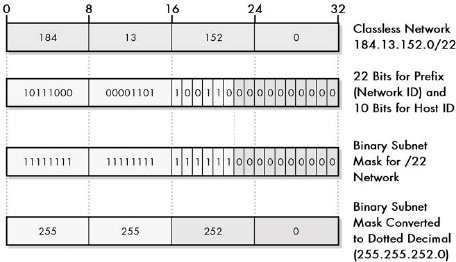
\includegraphics[width=.7\textwidth]{images/cidr-notation.jpg}
   \caption
      [CIDR (slash) notation and its subnet mask equivalent]
      {CIDR (slash) notation and its subnet mask equivalent -- A
      classless network is normally specified in CIDR, or slash notation, such
      as this example: 184.13.152.0/22. Here, the /22 means the first 22 bits
      of the address are the network ID. The equivalent subnet mask can be
      calculated by creating a 32-bit number with 22 ones followed by 10
      zeros.}
   \label{fig:cidr-notation}
\end{figure}


\begin{note}
You may recall that under classful subnetting, the bits used for
the subnet ID did not need to be contiguous. Even though this ability
was almost never used to avoid confusion, noncontiguous subnet ID bits
were possible. Under CIDR, the requirement for contiguous subnet ID bits
has been made official -- you could not use slash notation otherwise.
\end{note}

r

\section{Supernetting: subnetting the Internet}

In theory, then, what CIDR does is provide the central
address-assignment authority with the flexibility to hand out address
blocks of different sizes to organizations based on their need. However,
when CIDR was developed, a shift was made in the method by which public
IP addresses were assigned. Having everyone in the world attempt to get
addresses from one organization wasn't the best method. It was necessary
under the classful scheme because the hierarchy was only two levels
deep. The Internet Assigned Numbers Authority (IANA) handed out network
IDs to everyone, who then assigned host IDs (or subnetted).

Under CIDR, you have many hierarchical levels: You split big blocks into
smaller blocks, and then still-smaller blocks, and so on. It makes sense
to manage blocks in a similar hierarchical manner as well.
So what happens is that IANA/ICANN divides addresses into large blocks, which it distributes to the four \emph{regional Internet registries} (RIRs):
RIPE NCC (1992), APNIC (1993), ARIN (1997), and LACNIC (1999).%
   \footnote{AFRNIC was founded in 2004 as the fifth RIR.}
These then further divide the address blocks and distribute them to lower-level national Internet registries (NIRs),
local Internet registries (LIRs), and/or individual organizations such as Internet
service providers (ISPs).
This is all explained in the background discussion of Internet authorities and registries in {Chapter~3}.

ISPs can then divide these blocks into smaller ones and then allocate
them to their customers. These customers are sometimes smaller ISPs
themselves, which repeat the process. They split their blocks into
pieces of different sizes and allocate them to their customers, some of
whom are even smaller ISPs and some of whom are end users. The number of
times this can occur is limited only by how many addresses are in the
original block.

It's also worth noting that while CIDR is based on subnetting concepts,
subnetting itself is not used in CIDR -- or at least, not in the way it
is used under classful addressing. There is no explicit subnetting using
a subnet ID within CIDR. All IP addresses are interpreted only as having
a network ID and a host ID. An organization does the equivalent of
subnetting by dividing its own network into subnetworks using the same
general method that ISPs do. This probably seems a bit confusing. Later
in this chapter, I provide a detailed example of hierarchical address
block assignments and how splitting works under CIDR.



\section{Common aspects of classful and classless addressing}

There are a few aspects of addressing that were defined under the ``classful'' scheme that don't change under CIDR:
\begin{description}
   \item[Private address blocks]
      Certain blocks of addresses are still reserved for private network addressing.
      These addresses are not directly routed on the Internet, but can be used in conjunction with network address translation
      (NAT; see \cref{chap:nat}) to allow IP hosts without public addresses to access the Internet.

   \item[Addresses with special meanings]
      The special meanings assigned to certain network ID and host ID patterns are the same as before.
      This is also why you still must subtract two from the number of hosts in each network.
      These represent the all-zeros case that refers to the network as a whole and the all-ones address used for broadcast.

   \item[Loopback addresses]
      The network 127.0.0.0 is still reserved for loopback functionality.
      (In CIDR it is given the notation 127.0.0.0/8.)
\end{description}

Finally, note that use of classless addressing requires hardware and
software designed to handle it. If the hardware and software are still
assuming that they are operating in a classful environment, they will
not properly interpret addresses. Since CIDR has now been around for
more than a decade, this is usually not a problem with modern systems.



Because CIDR allows you to divide IP addresses into network IDs and host
IDs along any bit boundary, it allows for the creation of dozens of
different sizes of networks. As with subnetting, the size of network is
a trade-off between the number of bits used for the network ID and the
number used for the host ID. Unlike conventional subnetting, where a
single choice is made for all subnets, CIDR allows many levels of
hierarchical division of the Internet, so many sizes of networks exist
simultaneously. Larger networks are created and subdivided into smaller
ones.

Since many people are used to looking at IP address
blocks in terms of their classful sizes, it is common to express CIDR address
blocks in terms of their classful equivalents. First, at this point it
should be simple to see that a CIDR /8 network is equal in size to a
class A network, a /16 is equivalent to a class B network, and a/24 is
equivalent to a class C network. This is because class A networks use 8
bits for the network ID, class B networks use 16, and class C networks
use 24. However, remember that these CIDR equivalents do not need to
have any particular ranges for their first octets as in the classful
scheme.

Each time you reduce the prefix length, you are defining a network about
double the size of the one with the higher number, since you have
increased the number of bits in the host ID by one. So, a /15 network is
equal in size to two /16 networks.

%\protect\hyperlink{ch20s03.htmlux5cux23cidr_address_blocks_and_classful_address}{Table~20-1}
%shows each of the possible theoretical ways to divide the 32 bits of an
%IP address into network ID and host ID bits under CIDR. For each, I have
%shown the number of hosts in each network, and the way a network of each
%size is represented in both slash notation and as a conventional subnet
%mask. I have also shown the equivalent number of class A, class B, and
%class C networks for each.
%
%Keep the following things in mind while looking at this table:
%
%\begin{itemize}
%   \item
%      Some of the entries shown are more theoretical than practical and are
%      included merely for completeness. This is particularly the case with
%      the larger networks. For example, I doubt anyone ever actually works
%      with a /1 or /2 CIDR network; there would be only two of the former
%      and four of the latter encompassing the entire IP address space! Most
%      of the time, you will be working with smaller networks, /16 and below.
%   \item
%      Under normal circumstances, you cannot have a /31 or /32 CIDR network, because it would have zero valid host IDs.
%      (There is a special case: /31 networks can be used for point-to-point links, where it is obvious who the intended recipient is of each transmission,
%      and where broadcasts are not necessary.
%      This is described in RFC 3021.)
%   \item
%      In the columns showing the number of equivalent class A, B, and C networks I have only shown numbers in the range of 1/256 to 256 for simplicity.
%      Obviously, a /6 network, in addition to being equal in size to four class A networks, also equals 1,024 class B networks,
%      and 262,144 class C networks, but few people would bother referring to a /6 as being 262,144 class C networks.
%\end{itemize}

% The table is not useful.

The multiple hierarchical levels of CIDR make the technology seem rather
complicated. However, understanding how CIDR works really is not that
difficult, assuming you already know how subnetting is done. In
particular, if you know how VLSM functions, you basically already know
how CIDR works, since they are pretty much the same thing. They differ
only in the way that the hierarchical division of networks is
accomplished, and in the terminology.

To show how CIDR works better, let's take an example that will
illustrate the power of classless
addressing:
its ability to selectively subdivide a large block of addresses into
smaller ones that suit the needs of various organizations. Since address
allocation in CIDR typically starts with larger blocks owned by larger
ISPs, let's start there as well.

Suppose you have an ISP that is just starting up. It's not a major ISP,
but a moderate-sized one with only a few customers, so it needs only a
relatively small allocation. It begins with the block 71.94.0.0/15. The
/15 on the end of the block address tells you that this is a block of
addresses where the first 15 bits are the network ID and the last 17 are
the host ID. This block was obtained from a larger ISP, carved from a
larger block of addresses by that ISP. For example, 71.94.0.0/15 would
be equal to half of the address block 71.92.0.0/14, a quarter of the
block 71.88.0.0/13, and so on.

The ISP's block is equal in size to two class B networks and has a total
of 131,070 possible host addresses. This ISP can choose to divide this
block in a variety of ways, depending on the needs of its clients and
its own internal use. However, this ISP is just starting up, so it is
not even sure of what its ultimate needs will be. Let's say it expects
to resell about half of its address space to other ISPs, but isn't sure
what sizes they will need yet. Of the other half, it plans to split it
into four different sizes of blocks to match the needs of different-sized organizations.

To imagine how the ISP divides its address space, you can consider the analogy of cutting up a pie.
The ISP will first cut the pie in half and reserve one-half for its future ISP customers.
It will then cut the other half into some large pieces and some small pieces.
This is illustrated in \cref{fig:isp-divide-15}.
(Okay, I know it's a square pie. I wanted to show the individual small blocks to scale.)


\begin{figure}
   \centering
   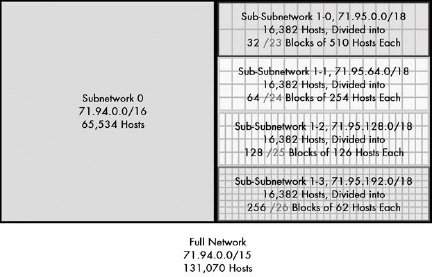
\includegraphics[width=.7\textwidth]{images/isp-divide-15.jpg}
   \caption
      [Example of a hierarchical division of a /15 CIDR address block]
      {Example of a hierarchical division of a /15 CIDR address block --
      This diagram shows one method by which an ISP with a relatively large /15 address block (131,070 hosts) might choose to hierarchically divide it.
      In this case it is first divided in half into two /16 blocks.
      One is reserved, while the other is divided into four /18 blocks.
      Each  of those is divided into blocks of a different size to allow allocation to organizations requiring up to 62, 126, 254, or 510 hosts, respectively.}
   \label{fig:isp-divide-15}
\end{figure}


The actual process of division might follow the progression described in the following section and illustrated in \cref{fig:cidr-hierarchical-division}.



\section{First level of division}

The ``pie'' is initially cut down the middle by using the single leftmost host ID bit as an extra network bit.
Here's the network address block, 71.94.0.0/15 in binary, with the leftmost host ID bit shown in bold:
\begin{quote}
0100 0111\quad 0101 111\textbf{0}\quad 0000 0000\quad 0000 0000
\end{quote}


To make the split, you make one network equal to this binary network
address with the highlighted bit remaining zero, and the other one with
it changed to a one. This creates two subnetworks -- not subnets as in
the classful sense of the word, but portions of the original
network -- that I have numbered based on the numeric value of what is
substituted into the new network ID bits, as follows:
\begin{itemize}
   \item Subnetwork 0: 0100 0111\quad 0101 111\textbf{0}\quad 0000 0000\quad 0000 0000
   \item Subnetwork 1: 0100 0111\quad 0101 111\textbf{1}\quad 0000 0000\quad 0000 0000
\end{itemize}

Because bit 16 is now also part of the network address, these are /16 networks, the size of a classful class B network.
So the subnetworks are as follows:
\begin{itemize}
   \item Subnetwork 0: 71.94.0.0/16
   \item Subnetwork 1: 71.95.0.0/16
\end{itemize}
You'll notice subnetwork 0 has the same IP address as the larger network it came from; this is always true of the subnetwork 0 in a network.


\begin{figure}
   \centering
   %\includegraphics{httpatomoreillycomsourcenostarchimages287849.png.jpg}
   \caption{Hierarchical address division using CIDR}
   \label{fig:cidr-hierarchical-division}
\end{figure}


\section{Second level of division}

Let's say you set aside subnetwork 0 earlier for future ISP allocations.
You then choose to divide the second subnetwork into four.
These you will then further subdivide into different sizes to meet the customer's needs.
To divide into four groups, you need two more bits from the host ID of subnetwork 1, as shown here in bold and underlined next to the original subnet bit:

\begin{longtable}[]{@{}l@{}}
\toprule
\endhead
01000111 0101111{\textbf{1 {00}}}000000 00000000\tabularnewline
\bottomrule
\end{longtable}

These two bits are replaced by the patterns 00, 01, 10, and 11 to get
four sub-subnetworks. They will be /18 networks, since you took two
extra bits from the host ID of a /16 as shown here:

\begin{longtable}[]{@{}l@{}}
\toprule
\endhead
Sub-subnetwork 1-0: 01000111 0101111{\textbf{1 {00}}}000000 00000000
(71.95.0.0/18)\tabularnewline
Sub-subnetwork 1-1: 01000111 0101111{\textbf{1 {01}}}000000 00000000
(71.95.64.0/18)\tabularnewline
Sub-subnetwork 1-2: 01000111 0101111{\textbf{1 {10}}}000000 00000000
(71.95.128.0/18)\tabularnewline
Sub-subnetwork 1-3: 01000111 0101111{\textbf{1 {11}}}000000 00000000
(71.95.192.0/18)\tabularnewline
\bottomrule
\end{longtable}

Each of these has 16,382 addresses.




\section{Third Level of Division}

You now take each of the four /18 networks and further subdivide it. You
want to make each of these contain a number of blocks of different sizes
corresponding to the potential customers. One way to do this would be as
follows:

{\textbf{Larger Organizations}} Customers needing up to 510 addresses
require a /23 network. You divide sub-subnetwork 1-0, 71.95.0.0/18 by
taking five bits from the host ID field:

\begin{longtable}[]{@{}l@{}}
\toprule
\endhead
01000111 0101111{\textbf{1 {00}}}{{00000}}0 00000000\tabularnewline
\bottomrule
\end{longtable}

You substitute into these five bits 00000, 00001, 00010 and so on,
giving you 32 different /23 networks in this block, each containing nine
bits for the host ID, for 510 hosts. The first will be
sub-sub-subnetwork 1-0-0, 71.95.0.0/23; the second sub-sub-subnetwork
1-0-1, 71.95.2.0/23; the last will be sub-sub-subnetwork 1-0-31:
71.95.62.0/23.

{\textbf{Medium-Sized Organizations}} For customers needing up to 254
addresses, you divide sub-subnetwork 1-1, 71.95.64.0/18, by taking six
bits from the host ID field:

\begin{longtable}[]{@{}l@{}}
\toprule
\endhead
01000111 0101111{\textbf{1 {01}}}{{000000}} 00000000\tabularnewline
\bottomrule
\end{longtable}

This gives you 64 different /24 networks. The first will be
sub-sub-subnetwork 1-1-0, 71.95.64.0/24, the second sub-sub-subnetwork
1-1-1, 71.95.65.0/24, and so on.

{\textbf{Smaller Organizations}} For customers with up to 126 hosts, you
divide sub-subnetwork 1-2, 71.95.128.0/18, by taking seven bits from the
host ID field, as follows:

\begin{longtable}[]{@{}l@{}}
\toprule
\endhead
01000111 0101111{\textbf{1}} {\textbf{{10}}}{{000000
0}}0000000\tabularnewline
\bottomrule
\end{longtable}

Seven bits allow 128 of these /25 networks within the /18 block. The
first will be 71.95.128.0/25, the second 71.95.128.128/25, the third
71.95.129.0/25, and so on.

{\textbf{Very Small Organizations}} For customers with up to 60 hosts,
you divide sub-subnetwork 1-3, 71.95.192.0/18, by taking eight bits from
the host ID field:

\begin{longtable}[]{@{}l@{}}
\toprule
\endhead
01000111 0101111{\textbf{1 {11}}}{{000000}} {{00}}000000\tabularnewline
\bottomrule
\end{longtable}

This gives you 256 different /26 networks within the /18 block. The
first will be 71.95.192.0/26, the second 71.95.192.64/26, and so on.

This example shows only one of many different ways to slice up this pie.
The ISP might decide that creating four different sizes of customer
networks in advance was not the right way to go. It might instead just
take the tack of dividing the pie in half, dividing it in half again,
and so on, as many times as needed to create slices of the right size.
Alternatively, if most of their customers needed around 50, 100, 200, or
500 hosts, the previous example might be the easiest to administer.

It would still be possible for the ISP to divide any of the smaller
blocks further if they needed to do so. They could split a /26
sub-sub-subnetwork into four /28 sub-sub-sub-subnetworks for very small
customers, for example. Also, an individual customer of this ISP could
do the same thing, dividing its own block to suit the internal structure
of its network.


